\documentclass[a4paper,12pt]{article}
\usepackage{amsmath} \usepackage{amsthm}
\usepackage[croatian]{babel}
\usepackage{graphicx}
\usepackage{amssymb} \usepackage{fancybox}
\usepackage{latexsym}
\usepackage{enumerate}
\usepackage[utf8]{inputenc}
\addtolength{\hoffset}{-1cm} \addtolength{\textwidth}{2cm}
\addtolength{\topmargin}{-2.8cm} \addtolength{\textheight}{3cm}

\newtheoremstyle{zad}% name
  {0.3cm}%      Space above
  {10pt}%      Space below
  {}%         Body font
  {}%         Indent amount (empty = no indent, \parindent = para indent)
  {\bf}% Thm head font
  {.}%        Punctuation after thm head
  {\newline}%     Space after thm head: " " = normal interword space;
        %       \newline = linebreak
  {}%         Thm head spec (can be left empty, meaning `normal')

\theoremstyle{zad}
\newtheorem{zadatak}{Zadatak}

\begin{document}
%\thispagestyle{empty}
\begin{center}
\shadowbox{\Large Lijepljenje torusa i deformiranih elipsoida}\\[2pt]
\end{center}
\bigskip
Torus je ploha koja ima implicitnu jednad\v{z}bu
$$\big(x^2+y^2+z^2+R^2-r^2\big)^2-4R^2\big(x^2+y^2\big)=0.$$
Za razli\v{c}ite odabire konstanti $R$ i $r$ dobivamo druk\v{c}ije toruse.\\[8pt]
Elipsoid je ploha koja ima implicitnu jednadžbu
\begin{equation*}
\frac{x^2}{a^2}+\frac{y^2}{b^2}+\frac{z^2}{c^2}-1=0.\tag{$\clubsuit$}
\end{equation*}
Stavimo li u ($\clubsuit$) npr. umjesto varijable $z$ izraz $z-\frac{1}{5}x^2$ dobivamo novu plohu s implicitnom jednadžbom
\begin{equation*}
\frac{x^2}{a^2}+\frac{y^2}{b^2}+\frac{\big(z-\frac{1}{5}x^2\big)^2}{c^2}-1=0
\end{equation*}
koju ćemo ovdje zvati deformirani elipsoid. Uz supstituciju $z-\frac{1}{5}x^2$ koristit ćemo ovdje i neke druge slične supstitucije i
u svakom od tih slučajeva pripadnu plohu zovemo deformirani elipsoid.\\[8pt]
Lijepljenjem torusa i deformiranih elipsoida možemo dobiti mnoge druge interesantne i egzotične plohe.
Proces lijepljenja ploha odgovara produktu njihovih implicitnih jednad\v{z}bi umanjenom za neku konstantu.\\[8pt]
Lijepljenjem dva deformirana elipsoida
\begin{gather*}
\frac{x^2}{25}+\frac{y^2}{0.25}+\frac{\big(z-\frac{1}{5}x^2\big)^2}{0.25}-1=0\text{\quad i\quad}
\frac{x^2}{0.25}+\frac{y^2}{25}+\frac{\big(z-\frac{1}{5}y^2\big)^2}{0.25}-1=0
\end{gather*}
dobivamo plohu prikazanu na slici \ref{sl1}.
Ta ploha ima implicitnu jednadžbu koja je jednaka produktu implicitnih jednadžbi zadanih ploha pri 
čemu je na kraju taj produkt još umanjen za konstantu $1$, tj.
$$\left(\frac{x^2}{25}+\frac{y^2}{0.25}+\frac{\big(z-\frac{1}{5}x^2\big)^2}{0.25}-1\right)\cdot
\left(\frac{x^2}{0.25}+\frac{y^2}{25}+\frac{\big(z-\frac{1}{5}y^2\big)^2}{0.25}-1\right)-1=0.$$
\begin{figure}[!h]
\centering
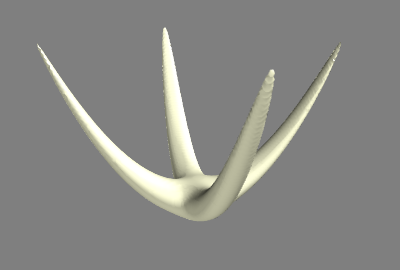
\includegraphics[scale=0.3]{cand1.png}
\vspace*{-5pt}
\caption{Lijepljenje dva deformirana elipsoida}\label{sl1}
\end{figure}
\pagebreak

\noindent Lijepljenjem dva deformirana elipsoida
\begin{align}
\frac{(x-5.05)^2}{2.25}+\frac{y^2}{0.04}+\frac{\big(z-5+\frac{1}{3}(x-5.05)^2\big)^2}{0.04}-1&=0\label{jed1}\\[5pt]
\frac{(x-5.05)^2}{0.04}+\frac{y^2}{2.25}+\frac{\big(z-5+\frac{1}{3}y^2\big)^2}{0.04}-1&=0\label{jed2}
\end{align}
i torusa ($R=1.8,\,r=0.2$)
\begin{equation}
\big((x-5.05)^2+y^2+(z-4.15)^2+R^2-r^2\big)^2-4R^2\big((x-5.05)^2+y^2\big)=0\label{jed3}
\end{equation}
dobivamo plohu prikazanu na slici \ref{sl2}.\par
\begin{figure}[!ht]
\centering
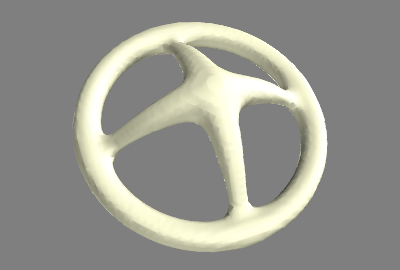
\includegraphics[scale=0.3]{cand2.png}
\vspace*{-5pt}
\caption{Lijepljenje dva deformirana elipsoida i torusa}\label{sl2}
\end{figure}
\noindent Preciznije, ta ploha ima implicitnu jednadžbu koja je jednaka produktu gornje tri implicitne jednadžbe zadanih ploha pri čemu je taj produkt umanjen za konstantu $40$.\\[8pt]
Lijepljenjem i translatiranjem ploha sa slika \ref{sl1} i \ref{sl2} dobivamo plohu prikazanu na slici \ref{sl3}.
\begin{figure}[!ht]
\centering
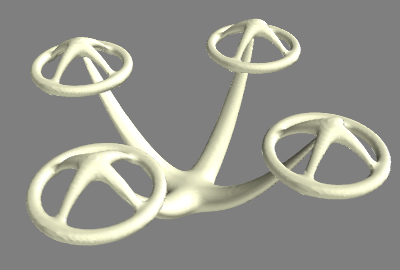
\includegraphics[scale=0.35]{cand3.png}
\vspace*{-5pt}
\caption{Lijepljenje ploha}\label{sl3}
\end{figure}


\end{document}



